% !TEX-encoding = UTF8

\documentclass[12pt,a4paper]{report}
\usepackage[T1]{fontenc}
\usepackage[utf8]{inputenc}
\usepackage[italian]{babel}

\usepackage{graphicx}
\usepackage{hyperref}

\usepackage[official]{eurosym}
\usepackage{listings}

\begin{document}
	
	\title
	{
		\huge{Benchmark Parallel BFS} \\
		\normalsize{Programmazione parallela} \\
		\rule{\linewidth}{2pt} \\  
		[0.5cm] 
	}
	\author{Nicolò Lutteri VR446688}
	\date{2021/10/11}
	
	\maketitle
	
	\tableofcontents
	
	\chapter{Introduzione}
	
		In questa breve relazione si è voluto analizzare le prestazioni dell'algoritmo BFS, in esecuzione sia in modo sequenziale sia su differenti schede grafiche.
		
	\chapter{Benchmark}
	
		I seguenti grafi sono stati generati da un'applicazione creata ad hoc.
		Mentre l'ultimo è stato scaricato dall'archivio "Standford Large Network DataSet Collection".
		Per ogni set viene viene variato il numero di THREAD BLOCK (che viene indicato nel titolo della sezione).
		
		\section{Hardware}
		
		L'hardware utilizzato è il seguente:
		
		\paragraph{PC Fisso}
		
			\begin{tabular}{|c|c|}
				\hline
				Processore & AMD Threadripper 1950X 16 Core (16/32) \\
				\hline
				RAM & 64GB \\
				\hline
				Scheda grafica & Nvidia 2080 Super \\
				\hline
				Spazio & 1TB NVMe \\
				\hline
			\end{tabular}
			
		\paragraph{Portatile}
		
			\begin{tabular}{|c|c|}
				\hline
				Processore & AMD Ryzen 7 3750H \\
				\hline
				RAM & 16GB \\
				\hline
				Scheda grafica & Nvidia 1660 Ti \\
				\hline
				Spazio & 512GB NVMe \\
				\hline
			\end{tabular}
		
		\section{Software}
		
			\paragraph{PC Fisso e portatile}
				
				\begin{tabular}{|c|c|}
					\hline
					Sistema operativo & Windows 10 \\
					\hline
					CUDA Toolkit & 11.0 \\
					\hline
					SM & 7.5 \\
					\hline
				\end{tabular}
			
		\section{Set-1}
		
			Ogni nodo è collegato con 1 altro nodo.
			Il peso del file è di 4MB.
		
			\begin{itemize}
				\item Nodi: 300.000
				\item Archi: 300.000
			\end{itemize}
		
		\subsection{16}
		
			\begin{tabular}{|c|c|c|}
				\hline
				Metodo & Tempo (Solo kernel) [ms] & Speed-up \\
				\hline
				Sequenziale & 11,54 & -  \\
				\hline
				2080 Super (No Shared) & 4,44 (1,52) & 3x \\
				\hline
				2080 Super (Shared) & 5,70 (2,76) & 2x \\
				\hline
			\end{tabular}
			
			\bigbreak
			
			\begin{tabular}{|c|c|c|}
				\hline
				PC Portatile & Tempo (Solo kernel) [ms] & Speed-up \\
				\hline
				Sequenziale & 12,66 & -  \\
				\hline
				1660 Ti (No Shared) & 5,73 (2,26) & 2x \\
				\hline
				1660 Ti (Shared) & 8,38 (4,94) & 2x \\
				\hline
			\end{tabular}

		\subsection{32}
		
			\begin{tabular}{|c|c|c|}
				\hline
				Metodo & Tempo (Solo kernel) [ms] & Speed-up \\
				\hline
				Sequenziale & 8,26 & -  \\
				\hline
				2080 Super (No Shared) & 4,73 (1,60) & 2x \\
				\hline
				2080 Super (Shared) & 5,08 (2,04) & 2x \\
				\hline
			\end{tabular}
			
			\bigbreak
			
			\begin{tabular}{|c|c|c|}
				\hline
				PC Portatile & Tempo (Solo kernel) [ms] & Speed-up \\
				\hline
				Sequenziale & 9,69 & -  \\
				\hline
				1660 Ti (No Shared) & 4,71 (1,54) & 2x \\
				\hline
				1660 Ti (Shared) & 6,12 (3,16) & 2x \\
				\hline
			\end{tabular}

		\subsection{64}
		
			\begin{tabular}{|c|c|c|}
				\hline
				Metodo & Tempo (Solo kernel) [ms] & Speed-up \\
				\hline
				Sequenziale & 7,73 & -  \\
				\hline
				2080 Super (No Shared) & 4,56 (1,35) & 2x \\
				\hline
				2080 Super (Shared) & 5,26 (1,76) & 1x \\
				\hline
			\end{tabular}
			
			\bigbreak
			
			\begin{tabular}{|c|c|c|}
				\hline
				PC Portatile & Tempo (Solo kernel) [ms] & Speed-up \\
				\hline
				Sequenziale & 7,07 & -  \\
				\hline
				1660 Ti (No Shared) & 5,46 (1,72) & 1x \\
				\hline
				1660 Ti (Shared) & 6,27 (2,49) & 1x \\
				\hline
			\end{tabular}

		\subsection{128}
		
			\begin{tabular}{|c|c|c|}
				\hline
				Metodo & Tempo (Solo kernel) [ms] & Speed-up \\
				\hline
				Sequenziale & 7,65 & -  \\
				\hline
				2080 Super (No Shared) & 4,30 (1,19) & 2x \\
				\hline
				2080 Super (Shared) & 4,53 (1,60) & 2x \\
				\hline
			\end{tabular}
			
			\bigbreak
			
			\begin{tabular}{|c|c|c|}
				\hline
				PC Portatile & Tempo (Solo kernel) [ms] & Speed-up \\
				\hline
				Sequenziale & 8,18 & -  \\
				\hline
				1660 Ti (No Shared) & 4,37 (1,35) & 2x \\
				\hline
				1660 Ti (Shared) & 4,62 (1,67) & 2x \\
				\hline
			\end{tabular}

		\subsection{256}
		
			\begin{tabular}{|c|c|c|}
				\hline
				Metodo & Tempo (Solo kernel) [ms] & Speed-up \\
				\hline
				Sequenziale & 7,38 & -  \\
				\hline
				2080 Super (No Shared) & 4,68 (1,32) & 2x \\
				\hline
				2080 Super (Shared) & 4,47 (1,40) & 2x \\
				\hline
			\end{tabular}
			
			\bigbreak
			
			\begin{tabular}{|c|c|c|}
				\hline
				PC Portatile & Tempo (Solo kernel) [ms] & Speed-up \\
				\hline
				Sequenziale & 7,23 & -  \\
				\hline
				1660 Ti (No Shared) & 5,14 (1,99) & 1x \\
				\hline
				1660 Ti (Shared) & 4,44 (1,52) & 2x \\
				\hline
			\end{tabular}
			
		\section{Set-2}
		
			Ogni nodo è collegato con altri 3 nodi.
			Il peso del file è di 80MB.
		
			\begin{itemize}
				\item Nodi: 5.000.000
				\item Archi: 5.000.000
			\end{itemize}
		
			\subsection{16}
			
				\begin{tabular}{|c|c|c|}
					\hline
					Metodo & Tempo (Solo kernel) [ms] & Speed-up \\
					\hline
					Sequenziale & 206,17 & -  \\
					\hline
					2080 Super (No Shared) & 41,02 (5,39) & 5x \\
					\hline
					2080 Super (Shared) & 61,23 (26,10) & 3x \\
					\hline
				\end{tabular}
				
				\bigbreak
				
				\begin{tabular}{|c|c|c|}
					\hline
					PC Portatile & Tempo (Solo kernel) [ms] & Speed-up \\
					\hline
					Sequenziale & 159,33 & -  \\
					\hline
					1660 Ti (No Shared) & 44,13 (11,16) & 4x \\
					\hline
					1660 Ti (Shared) & 89,05 (56,13) & 2x \\
					\hline
				\end{tabular}

			\subsection{32}
			
				\begin{tabular}{|c|c|c|}
					\hline
					Metodo & Tempo (Solo kernel) [ms] & Speed-up \\
					\hline
					Sequenziale & 198,99 & -  \\
					\hline
					2080 Super (No Shared) & 38,86 (5,16) & 5x \\
					\hline
					2080 Super (Shared) & 49,12 (14,74) & 4x \\
					\hline
				\end{tabular}
				
				\bigbreak
				
				\begin{tabular}{|c|c|c|}
					\hline
					PC Portatile & Tempo (Solo kernel) [ms] & Speed-up \\
					\hline
					Sequenziale & 159,88 & -  \\
					\hline
					1660 Ti (No Shared) & 43,29 (11,54) & 4x \\
					\hline
					1660 Ti (Shared) & 61,06 (31,10) & 3x \\
					\hline
				\end{tabular}

			\subsection{64}
			
				\begin{tabular}{|c|c|c|}
					\hline
					Metodo & Tempo (Solo kernel) [ms] & Speed-up \\
					\hline
					Sequenziale & 201,91 & -  \\
					\hline
					2080 Super (No Shared) & 40,76 (4,77) & 5x \\
					\hline
					2080 Super (Shared) & 42,62 (8,46) & 5x \\
					\hline
				\end{tabular}
				
				\bigbreak
				
				\begin{tabular}{|c|c|c|}
					\hline
					PC Portatile & Tempo (Solo kernel) [ms] & Speed-up \\
					\hline
					Sequenziale & 161,45 & -  \\
					\hline
					1660 Ti (No Shared) & 47,04 (11,53) & 3x \\
					\hline
					1660 Ti (Shared) & 47,65 (16,80) & 3x \\
					\hline
				\end{tabular}

			\subsection{128}
			
				\begin{tabular}{|c|c|c|}
					\hline
					Metodo & Tempo (Solo kernel) [ms] & Speed-up \\
					\hline
					Sequenziale & 198,28 & -  \\
					\hline
					2080 Super (No Shared) & 39,43 (4,65) & 5x \\
					\hline
					2080 Super (Shared) & 39,24 (4,91) & 5x \\
					\hline
				\end{tabular}
				
				\bigbreak
				
				\begin{tabular}{|c|c|c|}
					\hline
					PC Portatile & Tempo (Solo kernel) [ms] & Speed-up \\
					\hline
					Sequenziale & 140,01 & -  \\
					\hline
					1660 Ti (No Shared) & 41,74 (10,28) & 3x \\
					\hline
					1660 Ti (Shared) & 41,04 (9,74) & 3x \\
					\hline
				\end{tabular}

			\subsection{256}
			
				\begin{tabular}{|c|c|c|}
					\hline
					Metodo & Tempo (Solo kernel) [ms] & Speed-up \\
					\hline
					Sequenziale & 208,01 & -  \\
					\hline
					2080 Super (No Shared) & 40,34 (5,09) & 5x \\
					\hline
					2080 Super (Shared) & 39,72 (3,92) & 5x \\
					\hline
				\end{tabular}
				
				\bigbreak
				
				\begin{tabular}{|c|c|c|}
					\hline
					PC Portatile & Tempo (Solo kernel) [ms] & Speed-up \\
					\hline
					Sequenziale & 158,29 & -  \\
					\hline
					1660 Ti (No Shared) & 40,86 (9,98) & 4x \\
					\hline
					1660 Ti (Shared) & 37,91 (6,92) & 4x \\
					\hline
				\end{tabular}
			
		\section{Set-3}
		
			Ogni nodo è collegato con altri 10 nodi.
			Il peso del file è di 1,8GB.
		
			\begin{itemize}
				\item Nodi: 100.000.000
				\item Archi: 100.000.000
			\end{itemize}
	
			\subsection{16}
			
				\begin{tabular}{|c|c|c|}
					\hline
					Metodo & Tempo (Solo kernel) [ms] & Speed-up \\
					\hline
					Sequenziale & 4268,86 & -  \\
					\hline
					2080 Super (No Shared) & 770,35 (64,56) & 6x \\
					\hline
					2080 Super (Shared) & 966,59 (271,26) & 4x \\
					\hline
				\end{tabular}
				
				\bigbreak
				
				\begin{tabular}{|c|c|c|}
					\hline
					PC Portatile & Tempo (Solo kernel) [ms] & Speed-up \\
					\hline
					Sequenziale & 3433,98 & -  \\
					\hline
					1660 Ti (No Shared) & 728,92 (143,79) & 5x \\
					\hline
					1660 Ti (Shared) & 1147,55 (559,06) & 3x \\
					\hline
				\end{tabular}

			\subsection{32}
			
				\begin{tabular}{|c|c|c|}
					\hline
					Metodo & Tempo (Solo kernel) [ms] & Speed-up \\
					\hline
					Sequenziale & 4296,15 & -  \\
					\hline
					2080 Super (No Shared) & 895,62 (160,09) & 5x \\
					\hline
					2080 Super (Shared) & 867,98 (143,92) & 5x \\
					\hline
				\end{tabular}
				
				\bigbreak
				
				\begin{tabular}{|c|c|c|}
					\hline
					PC Portatile & Tempo (Solo kernel) [ms] & Speed-up \\
					\hline
					Sequenziale & 3286,99 & -  \\
					\hline
					1660 Ti (No Shared) & 856,52 (258,87) & 4x \\
					\hline
					1660 Ti (Shared) & 914,49 (293,19) & 4x \\
					\hline
				\end{tabular}

			\subsection{64}
			
				\begin{tabular}{|c|c|c|}
					\hline
					Metodo & Tempo (Solo kernel) [ms] & Speed-up \\
					\hline
					Sequenziale & 4315,78 & -  \\
					\hline
					2080 Super (No Shared) & 870,72 (167,40) & 5x \\
					\hline
					2080 Super (Shared) & 809,46 (76,55) & 5x \\
					\hline
				\end{tabular}
				
				\bigbreak
				
				\begin{tabular}{|c|c|c|}
					\hline
					PC Portatile & Tempo (Solo kernel) [ms] & Speed-up \\
					\hline
					Sequenziale & 3007,07 & -  \\
					\hline
					1660 Ti (No Shared) & 887,65 (296,81) & 3x \\
					\hline
					1660 Ti (Shared) & 751,20 (157,93) & 4x \\
					\hline
				\end{tabular}

			\subsection{128}
			
				\begin{tabular}{|c|c|c|}
					\hline
					Metodo & Tempo (Solo kernel) [ms] & Speed-up \\
					\hline
					Sequenziale & 4367,78 & -  \\
					\hline
					2080 Super (No Shared) & 870,05 (162,37) & 5x \\
					\hline
					2080 Super (Shared) & 766,99 (49,17) & 6x \\
					\hline
				\end{tabular}
				
				\bigbreak
				
				\begin{tabular}{|c|c|c|}
					\hline
					PC Portatile & Tempo (Solo kernel) [ms] & Speed-up \\
					\hline
					Sequenziale & 3316,59 & -  \\
					\hline
					1660 Ti (No Shared) & 886,58 (285,93) & 4x \\
					\hline
					1660 Ti (Shared) & 685,65 (96,09) & 5x \\
					\hline
				\end{tabular}

			\subsection{256}
			
				\begin{tabular}{|c|c|c|}
					\hline
					Metodo & Tempo (Solo kernel) [ms] & Speed-up \\
					\hline
					Sequenziale & 4343 & -  \\
					\hline
					2080 Super (No Shared) & 848,40 (154,80) & 5x \\
					\hline
					2080 Super (Shared) & 744,30 (39,25) & 6x \\
					\hline
				\end{tabular}
				
				\bigbreak
				
				\begin{tabular}{|c|c|c|}
					\hline
					PC Portatile & Tempo (Solo kernel) [ms] & Speed-up \\
					\hline
					Sequenziale & 3215,89 & -  \\
					\hline
					1660 Ti (No Shared) & 959,16 (283,42) & 3x \\
					\hline
					1660 Ti (Shared) & 665,48 (86,71) & 5x \\
					\hline
				\end{tabular}

		\section{roadNet-CA}
		
			Grafo che rappresenta le connessione delle strade in California.
			Il peso del file è di 90MB.
		
			\begin{itemize}
				\item Nodi: 1.965.206
				\item Archi: 5.533.214
			\end{itemize}
				
			\subsection{16}
			
			\begin{tabular}{|c|c|c|}
					\hline
					Metodo & Tempo (Solo kernel) [ms] & Speed-up \\
					\hline
					Sequenziale & 118,12 & -  \\
					\hline
					2080 Super (No Shared) & 127,61 (109,87) & 0,9x \\
					\hline
					2080 Super (Shared) & 305,49 (287,96) & 0,4x \\
					\hline
				\end{tabular}
				
				\bigbreak
				
				\begin{tabular}{|c|c|c|}
					\hline
					PC Portatile & Tempo (Solo kernel) [ms] & Speed-up \\
					\hline
					Sequenziale & 87,26 & -  \\
					\hline
					1660 Ti (No Shared) & 202,17 (186,26) & 0,4x \\
					\hline
					1660 Ti (Shared) & 506,50 (490,05) & 0,2x \\
					\hline
				\end{tabular}
			
			\subsection{32}
			
				\begin{tabular}{|c|c|c|}
					\hline
					Metodo & Tempo (Solo kernel) [ms] & Speed-up \\
					\hline
					Sequenziale & 117,06 & -  \\
					\hline
					2080 Super (No Shared) & 95,97 (78,66) & 1x \\
					\hline
					2080 Super (Shared) & 199,88 (182,06) & 0,6x \\
					\hline
				\end{tabular}
				
				\bigbreak
				
				\begin{tabular}{|c|c|c|}
					\hline
					PC Portatile & Tempo (Solo kernel) [ms] & Speed-up \\
					\hline
					Sequenziale & 100,16 & -  \\
					\hline
					1660 Ti (No Shared) & 131,48 (115,42) & 0,8x \\
					\hline
					1660 Ti (Shared) & 322,86 (306,81) & 0,3x \\
					\hline
				\end{tabular}

			\subsection{64}
			
				\begin{tabular}{|c|c|c|}
					\hline
					Metodo & Tempo (Solo kernel) [ms] & Speed-up \\
					\hline
					Sequenziale & 123,30 & -  \\
					\hline
					2080 Super (No Shared) & 82,52 (65,00) & 1x \\
					\hline
					2080 Super (Shared) & 134,00 (116,91) & 0,9x \\
					\hline
				\end{tabular}
				
				\bigbreak
				
				\begin{tabular}{|c|c|c|}
					\hline
					PC Portatile & Tempo (Solo kernel) [ms] & Speed-up \\
					\hline
					Sequenziale & 86,05 & -  \\
					\hline
					1660 Ti (No Shared) & 125,49 (108,67) & 0,7x \\
					\hline
					1660 Ti (Shared) & 195,54 (179,78) & 0,4x \\
					\hline
				\end{tabular}

			\subsection{128}
			
				\begin{tabular}{|c|c|c|}
					\hline
					Metodo & Tempo (Solo kernel) [ms] & Speed-up \\
					\hline
					Sequenziale & 115,36 & -  \\
					\hline
					2080 Super (No Shared) & 76,27 (58,66) & 2x \\
					\hline
					2080 Super (Shared) & 99,57 (82,42) & 1x \\
					\hline
				\end{tabular}
				
				\bigbreak
				
				\begin{tabular}{|c|c|c|}
					\hline
					PC Portatile & Tempo (Solo kernel) [ms] & Speed-up \\
					\hline
					Sequenziale & 87,58 & -  \\
					\hline
					1660 Ti (No Shared) & 79,25 (63,48) & 1x \\
					\hline
					1660 Ti (Shared) & 139,89 (124,26) & 0,6x \\
					\hline
				\end{tabular}

			\subsection{256}
			
				\begin{tabular}{|c|c|c|}
					\hline
					Metodo & Tempo (Solo kernel) [ms] & Speed-up \\
					\hline
					Sequenziale & 114,28 & -  \\
					\hline
					2080 Super (No Shared) & 79,27 (61,44) & 1x \\
					\hline
					2080 Super (Shared) & 94,84 (77,34) & 1x \\
					\hline
				\end{tabular}
				
				\bigbreak
				
				\begin{tabular}{|c|c|c|}
					\hline
					PC Portatile & Tempo (Solo kernel) [ms] & Speed-up \\
					\hline
					Sequenziale & 89,62 & -  \\
					\hline
					1660 Ti (No Shared) & 76,04 (60,48) & 1x \\
					\hline
					1660 Ti (Shared) & 110,32 (94,17) & 0,8x \\
					\hline
				\end{tabular}
			
			\subsection{Analisi}
			
				Analisi effettuata con il tool Nvidia Nsight System, con numero di THREAD BLOCK pari a 256.
				
				\begin{center}
					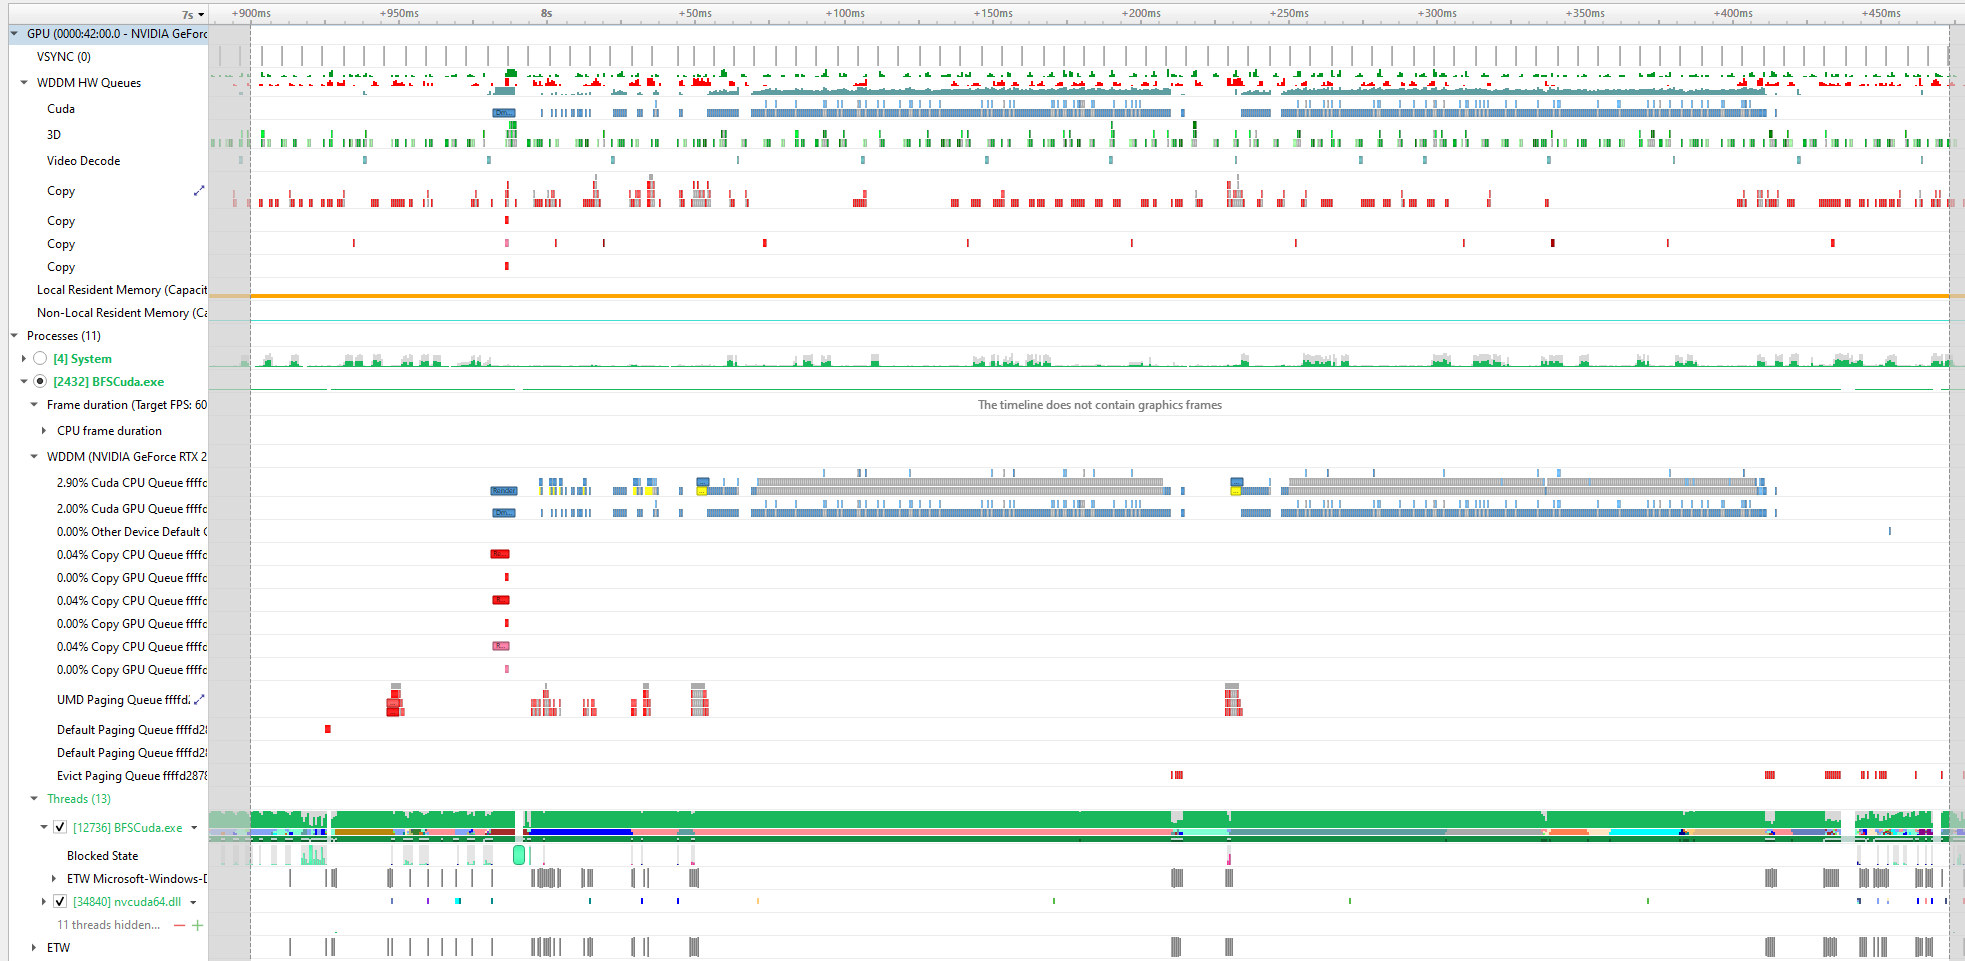
\includegraphics[width=1\linewidth]{Tool}
				\end{center}
	
\end{document}
